\documentclass[12pt]{article}
\usepackage[a4paper]{geometry}
\usepackage[utf8]{inputenc}
\usepackage{fancyhdr}
\usepackage{lastpage}
\usepackage{graphicx, wrapfig, subcaption, setspace, booktabs}
\usepackage{graphicx}
\usepackage[T1]{fontenc}
\usepackage[font=small, labelfont=bf]{caption}
\usepackage[protrusion=true, expansion=true]{microtype}
\usepackage[english]{babel}
\usepackage{sectsty}
\usepackage{url, lipsum}
\usepackage[T1]{fontenc}
\usepackage{icomma}
\usepackage{siunitx}
\usepackage{ragged2e}
\usepackage{amsmath}
\usepackage{comment}
\usepackage{enumerate}
\usepackage{anysize}


\newcommand{\HRule}[1]{\rule{\linewidth}{#1}}
\onehalfspacing
\setcounter{tocdepth}{5}
\setcounter{secnumdepth}{5}

\begin{document}

\begin{titlepage}

\title{ \normalsize 
        \begin{center}
        
\includegraphics[height=6cm]{logo.png}
        \end{center}
        \LARGE \textsc{\textbf{Universidad De Sonora}} \\ \bigskip
		\Large División de Ciencias Exactas y Naturales \\
        Licenciatura en Física \\ \bigskip
        \bigskip
        Física Computacional I
		\\ [0.1cm]  
		\HRule{2pt} \\
		\Large \textbf{{Actividad 7}} \\
        \textit{\textbf{"Sistema de resortes acoplados Final"}}
		\HRule{2pt} \\
		\normalsize \vspace*{0.001\baselineskip}}
        
\date{\bigskip \Large Hermosillo, Sonora  \hspace*{\fill}  24 de Marzo de 2018}

        
\author{
		\Large\textbf{ Michelle Contreras Cossio} \\ \bigskip
        \\ \bigskip
       \Large Profr. Carlos Lizárraga Celaya}
       \end{titlepage}
       \maketitle
       

\newpage
\pagestyle{plain}

\section{Introducción}
El presente reporte muestra el procedimiento y resultados obtenidos al realizar la actividad \#7 de la clase Física Computacional I.  Durante esta práctica se retoma el artículo utilizado en la práctica anterior, continuando con los siguientes apartados, por lo que el objetivo prevalece el cual es continuar con el uso de Python, enfocándonos en la simulación de cierto fenómeno físico, para poder comparar soluciones numéricas con analíticas. \\

De igual manera, continuaremos trabajando con jupyter lab utilizando el archivo de "Coupled spring equations", trabajando con el sistema de resortes acoplados ya sea sencillo, con amortiguamiento, con algún coeficiente no lineal y con fuerzas externas.\\

A continuación se presenta la síntesis completa del artículo. 

\section{Síntesis de "Coupled spring equations"}

En esta sección mostramos una síntesis de artículo "Coupled spring equations" por Temple H. Fay y Sarah Duncan Graham. Además se añade el código utilizado para resolver estos mismos problemas, haciendo uso de jupyter lab.

\subsection{Introducción}
En este artículo, se trata el problema de dos resortes y dos masas, conectados en serie y suspendidos desde el techo. Para resolver este fenómeno, se hace uso de la Ley de Hooke, para la fuerza restauradora del resorte, lo que resulta en la solución de ecuaciones diferenciales lineales de segundo orden, sin embargo, se pueden llegar a convertir en ecuaciones diferenciales lineales de hasta cuarto orden.\\ 

A partir de estas ecuaciones se pueden tener muchas interpretaciones físicas, sobre la fase o desfase, además que se pueden agregar términos como uno no lineal, que pretende mostrar algo físicamente más viable. \\

En resumen, podemos modificar fácilmente variables como la periodicidad, fase, amplitud, entre otras, modificando simplemente las ecuaciones.

\subsection{El modelo de resortes acoplados}

Este modelo consiste en dos resortes y dos masas, valores de k y m diferentes, colgados al techo y movidos desde su posición de equilibrio en x. 

\subsubsection{Asumiendo la Ley de Hooke}

Tomando como cierta la Ley de Hooke, cada resorte estirados tendrá una fuerza restauradora de -kx, donde k es la constante del resorte y x es lo que se estiró. 

\begin{center}
        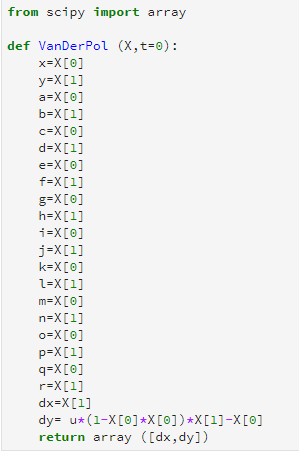
\includegraphics[height=6cm]{1.png}
\end{center}

La masa superior siente dos fuerzas, puesto que se encuentra entre dos resortes, la propia al resorte superior y una fuerza hacia arriba por la resistencia del segundo resorte para ser estirado. Mientras que la masa inferior únicamente siente la fuerza del resorte al cual se encuentra conectado. De esta manera, gracias a la Ley de Newton, podemos representar lo dicho en dos ecuaciones:

\begin{equation}
m_1 \ddot x_1 = -k_1x_1 - k_2(x_1-x_2)
\end{equation}

\begin{equation}
m_2 \ddot x_2 = -k_2(x_2-x_1)
\end{equation}

Si se buscara encontrar una ecuación para $x_1$, de modo que no se involucrara a $x_2$, y viceversa se obtienen dos ecuaciones lineales de cuarto grado, a las cuales se llega, despejando una variable de la primera ecuación y sustituyendo en la segunda:\\

\centerline{$m_1m_2x_1^{(4)} + (m_2k_1 + k_2(m_1+m_2)) \ddot x_1 + k_1k_2x_1=0$}
\centerline{$m_1m_2x_2^{(4)} + (m_2k_1 + k_2(m_1+m_2)) \ddot x_2 + k_1k_2x_2=0$}
.\\
Ecuaciones con las cuales, solamente se hace uso de los desplazamientos y velocidades iniciales. Así pues, una alternativa que se tiene es convertir el sistema de dos ecuaciones de segundo orden a uno de 4 ecuaciones de cuarto orden. Sin embargo, en los ejemplos se trabajara con el primer sistema. 

\subsubsection{Ejemplos} 
Los siguientes ejemplos muestran el uso de dos masas $m_1$ = $m_2$ = 1. Sin fricción ni fuerza externa, haciendo uso de las ecuaciones (1) y (2).

\begin{itemize}
\item \textbf{Ejemplo 2.1}

Describir el movimiento de los resortes con $k_1$=6, $k_2$=4 y condiciones iniciales $(x_1(0), \dot x_1(0), x_2(0), \dot x_2(0))$ = (1, 0, 2, 0).\\

Resolviendo las ecuaciones, se llegó a que la solución analítica para este problema es: \\

\centerline{$x_1(t) = cos\sqrt (2t)$}
\centerline{$x_2(t) = 2cos\sqrt (2t)$}

Este movimiento es sincronizado y se encuentra en fase, las masas tienen el mismo período, esto se puede ver en la gráficas creadas, mostradas a continuación. 

\begin{itemize}
\item \textbf{Solución numérica con Python:}

NOTA: El código mostrado a continuación, así como el que produce las gráficas, se utilizó de manera idéntica para los ejemplos 2.1, 2.2 y 2.3, cambiando únicamente las condiciones iniciales (celda 2):

Lo que hace este código es crear vectores que obtengan los valores para las velocidades, posiciones, masas, constantes de los resortes, etc.

\begin{center}
        
\includegraphics[height=6cm]{2.png}
\end{center}

Posteriormente se tiene una sección que permite dar los valores iniciales de masas, constantes, etc. Se crea un archivo de datos, con tiempos que van cambiando según se asigne, que contiene tiempos, velocidad y posición a cierto tiempo y el error (en este caso y en el ejemplo 2.2). 

\begin{center}
        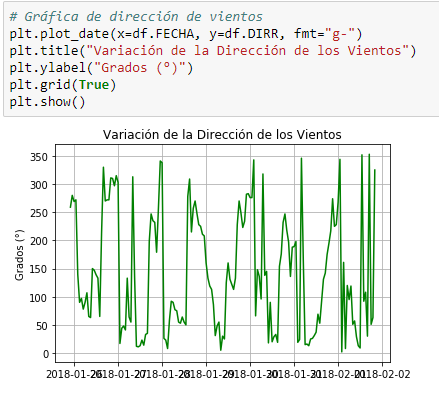
\includegraphics[height=14cm]{3.png}
\end{center}


A partir de ese archivo se crearon las gráficas, utilizando algunas de las variables que contenga. 

\clearpage
Así se produjo el movimiento de $x_1$ y de $x_2$ a través del tiempo:

\begin{center}
        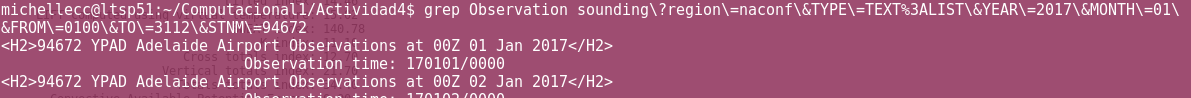
\includegraphics[height=7cm]{4.png}
\end{center}

Dando como resultado:

\begin{center}
        \includegraphics[height=6cm]{ej2_1_1.png}
\end{center}


Así se produjo la fase de $x_1$ y de $x_2$ (v vs x):

\begin{center}
        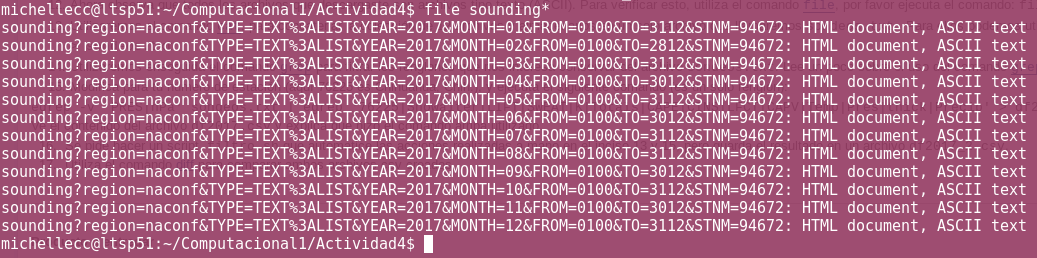
\includegraphics[height=7cm]{5.png}
\end{center}

Dando como resultado:

\begin{center}
        \includegraphics[height=6cm]{ej2_1_2.png}
\end{center}

Así se produjo $x_1$ y vs $x_2$:

\begin{center}
        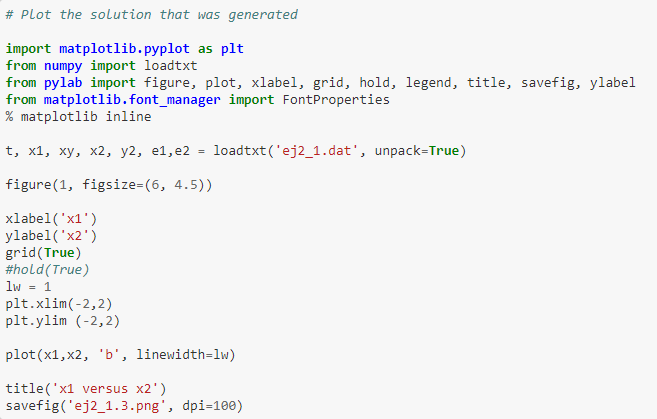
\includegraphics[height=7cm]{6.png}
\end{center}

Dando como resultado:


\begin{center}
        \includegraphics[height=6cm]{ej2_1_3.png}
\end{center}

\item \textbf{Calculo del error}

Para calcular el error, primeramente, se agregaron al archivo creado dos columnas,una para el error con respecto a $x_1$ y otra para el error con respecto a $x_2$, esos errores se calcularon restando a la x correspondiente a cierto tiempo (valor numérico), la función solución evaluada en el mismo tiempo (valor analítico),y dividiendolo entre este valor analítico. 


\begin{center}
        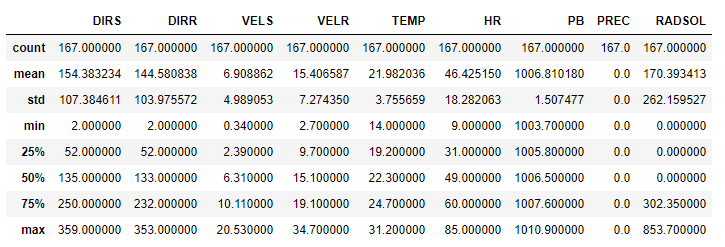
\includegraphics[height=2cm]{7.png}
\end{center}

\begin{center}
        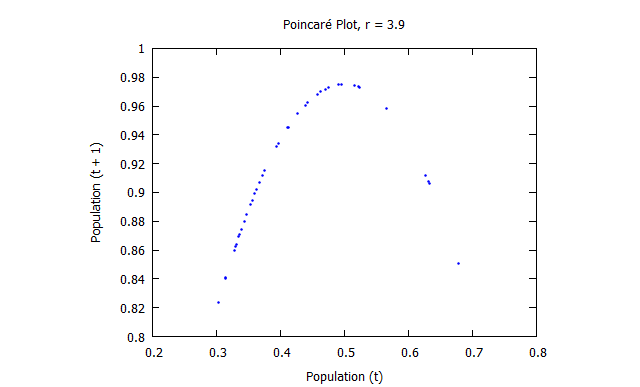
\includegraphics[height=7cm]{8.png}
\end{center}

Posteriormente, se graficaron ambos errores con respecto del tiempo:

\begin{center}
        \includegraphics[height=6cm]{error2_1.png}
\end{center}

\end{itemize}

\item \textbf{Ejemplo 2.2}

Describir el movimiento de los resortes con $k_1$=6, $k_2$=4 y condiciones iniciales $(x_1(0), \dot x_1(0), x_2(0), \dot x_2(0))$ = (-2, 0, 1, 0).\\

Resolviendo las ecuaciones, se llegó a que la solución analítica para este problema es: \\

\centerline{$x_1(t) = -2cos (2\sqrt (3t))$}
\centerline{$x_2(t) = cos (2\sqrt (3t))$}

Lo que representa que cuando una masa se mueve para arriba, la otra se mueve para abajo, pero tienen el mismo período, con un desfase de 180$^\circ$

\begin{itemize}
\item \textbf{Solución numérica con Python}

Se utilizó el mismo código utilizado en el ejemplo anterior, pero únicamente se produjeron las gráficas de el movimiento de $x_1$ y de $x_2$ a través del tiempo:


\begin{center}
        \includegraphics[height=6cm]{ej2_2_1.png}
\end{center}

y de $x_1$ y vs $x_2$:


\begin{center}
        \includegraphics[height=6cm]{ej2_2_2.png}
\end{center}

\item \textbf{Cálculo del error}
\end{itemize}

El error se produjo de la misma manera que en el ejemplo anterior, utilizando ahora las nuevas soluciones analíticas, la gráfica obtenida fue la siguiente:


\begin{center}
        \includegraphics[height=6cm]{error2_2.png}
\end{center}

\item \textbf{Ejemplo 2.3}

Describir el movimiento de los resortes con $k_1$=0.4, $k_2$=1.808 y condiciones iniciales $(x_1(0), \dot x_1(0), x_2(0), \dot x_2(0))$ = (1/2, 0, -1/2, 7/10).\\

Cambiando estos valores iniciales, únicamente va a cambiar el período y la frecuencia, así como la amplitud y fase en la soluciones. Con los programas que creamos podemos verificar eso al variar los valores de k. 

\begin{itemize}
\item \textbf{Solución numérica con Python}

Se realizaron básicamente las mismas gráficas que se crearon en los ejemplos anteriores.

Primeramente se crearon las gráficas de fase, una para $x_1$ y otra para $x_2$, esta vez se encuentra cada uno en una gráfica.

\begin{figure}[h!]
\begin{subfigure}{.55\textwidth}
\centering
\includegraphics[width=1\linewidth]{ej2_3_1.png}
\end{subfigure}
\begin{subfigure}{.55\textwidth}
\centering
\includegraphics[width=1\linewidth]{ej2_3_2.png}
\end{subfigure}
\end{figure}

\clearpage
Posteriormente el plot de $x_1$ y $x_2$, por separado con respecto al tiempo. 

\begin{figure}[h!]
\begin{subfigure}{.55\textwidth}
\centering
\includegraphics[width=1\linewidth]{ej2_3_3.png}
\end{subfigure}
\begin{subfigure}{.55\textwidth}
\centering
\includegraphics[width=1\linewidth]{ej2_3_4.png}
\end{subfigure}
\end{figure}

El movimiento de $x_1$ y $x_2$ con respecto al tiempo, en una sola.

\begin{center}
        \includegraphics[height=6cm]{ej2_3_5.png}
\end{center}

Plot de $x_1$ vs $x_2$.

\begin{center}
        \includegraphics[height=6cm]{ej2_3_6.png}
\end{center}

\end{itemize}


\end{itemize}

\subsubsection{Amortiguamiento}
El tipo de amortiguamiento (o fricción para el caso en el que las masas se encuentran sobre alguna superficie) con el que estaremos trabajando es el viscoso, que depende únicamente de la velocidad. En este caso, que tenemos dos resortes, el amortiguamiento de la primera masa depende únicamente de su velocidad y no de la velocidad de la otra masa y viceversa. \\

Así, añadiendo el término de amortiguamiento, las ecuaciones quedan:

\begin{equation}
m_1 \ddot x_1 = -\delta _1 \dot{x_1} -k_1x_1 - k_2(x_1-x_2)
\end{equation}
\begin{equation}
m_2 \ddot x_2 = -\delta _2 \dot{x_2} -k_2(x_2-x_1)
\end{equation}

De igual manera que en el movimiento de dos resortes acoplados simples, se puede modificar el sistema que tenemos de dos ecuaciones de segundo grado a un sistema de cuatro ecuaciones de cuarto grado, sin embargo, trabajaremos con el que ya tenemos. 

\begin{itemize}
\item \textbf{Ejemplo 2.4}

Describir el movimiento de los resortes con $m_1 = m_2 = 1$, $k_1$=0.4, $k_2$=1.808, constantes de amortiguamiento $\delta _1$= 0.1, $\delta _2$= 0.2 y condiciones iniciales $(x_1(0), \dot x_1(0), x_2(0), \dot x_2(0))$ = (1, 1/2, 2, 1/2).

El amortiguamiento va a causar que poco a poco la amplitud del movimiento disminuya. 

\begin{itemize}
\item \textbf{Solución numérica con Python}

El código utilizado sigue siendo el mismo, únicamente se tiene que en este caso si existirán coeficientes de fricción/ amortiguamiento.
Se crearon las mismas gráficas del ejemplo anterior.

Gráficas de fase, una para $x_1$ y otra para $x_2$.

\begin{figure}[h!]
\begin{subfigure}{.45\textwidth}
\centering
\includegraphics[width=1\linewidth]{ej2_4_1.png}
\end{subfigure}
\begin{subfigure}{.45\textwidth}
\centering
\includegraphics[width=1\linewidth]{ej2_4_1.png}
\end{subfigure}
\end{figure}

Plot de $x_1$ y $x_2$
\begin{figure}[h!]
\begin{subfigure}{.55\textwidth}
\centering
\includegraphics[width=1\linewidth]{ej2_4_3.png}
\end{subfigure}
\begin{subfigure}{.55\textwidth}
\centering
\includegraphics[width=1\linewidth]{ej2_4_4.png}
\end{subfigure}
\end{figure}

El movimiento de $x_1$ y $x_2$ con respecto al tiempo

\begin{center}
        \includegraphics[height=6cm]{ej2_4_5.png}
\end{center}

Plot de $x_1$ vs $x_2$.

\begin{center}
        \includegraphics[height=6cm]{ej2_4_6.png}
\end{center}

\end{itemize}

\end{itemize}

\subsection{Agregando no linealidad}

Si asumimos que las fuerzas de restauración son no lineales, que es muy probable si nos aproximamos a un sistema real, se modifican las ecuaciones que teniamos, de la siguiente manera: 

\begin{equation}
m_1 \ddot x_1 = -\delta _1 \dot{x_1} -k_1x_1 +\mu _1 x_1 ^3- k_2(x_1-x_2) + \mu _2 (x_1-x_2)^3
\end{equation}
\begin{equation}
m_2 \ddot x_2 = -\delta _2 \dot{x_2} -k_2(x_2-x_1) +\mu _2 (x_2-x_1)^3
\end{equation} 

Sin embargo, este modelo es mucho más complicado que uno lineal, tanto que si tomamos intervalos de tiempo grandes, las soluciones numéricas dejan de acercarse a la solución real. 

\begin{itemize}
\item \textbf{Ejemplo 3.1}

Describir el movimiento de los resortes con $m_1 = m_2 = 1$, $k_1$=0.4, $k_2$=1.808, constantes de amortiguamiento $\delta _1$= 0, $\delta _2$= 0, coeficientes no lineales $\mu _1$=-1/6, $\mu _2$=-1/10 y condiciones iniciales $(x_1(0), \dot x_1(0), x_2(0), \dot x_2(0))$ = (1, 0, -1/2, 0).

El movimiento es oscilatorio y parece periódico, no hay amortiguamiento que disminuya la amplitud, aparentemente tienen un desfase de 180$^\circ$, debido que es no lineal, el modelo tiene sensibilidad a las condiciones iniciales. 

\begin{itemize}
\item \textbf{Solución numérica con Python}

El código utilizado fue básicamente el mismo que el mostrado en el ejemplo 2.1, a continuación se muestran las modificaciones a tal código (utilizado también en el ejemplo 3.2 y 3.3:

\begin{center}
        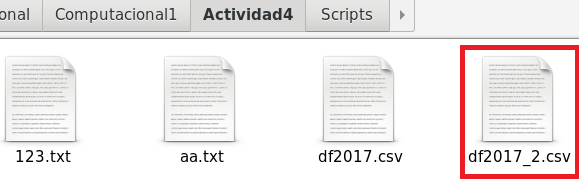
\includegraphics[height=6cm]{9.png}
\end{center}

\begin{center}
        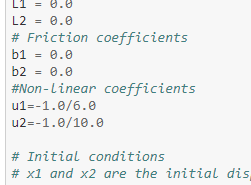
\includegraphics[height=3cm]{10.png}
\end{center}

Y claramente, cada vez que se mencionara al vector p, se agregaron las variables u1 y u2.

Las gráficas que se crearon, fueron las mismas que en los ejemplos anteriores, por lo que el código es análogo. Gráficas de fase, una para $x_1$ y otra para $x_2$.

\begin{figure}[h!]
\begin{subfigure}{.55\textwidth}
\centering
\includegraphics[width=1\linewidth]{ej3_1_1.png}
\end{subfigure}
\begin{subfigure}{.55\textwidth}
\centering
\includegraphics[width=1\linewidth]{ej3_1_2.png}
\end{subfigure}
\end{figure}

Plot de $x_1$ y $x_2$

\begin{figure}[h!]
\begin{subfigure}{.55\textwidth}
\centering
\includegraphics[width=1\linewidth]{ej3_1_3.png}
\end{subfigure}
\begin{subfigure}{.55\textwidth}
\centering
\includegraphics[width=1\linewidth]{ej3_1_4.png}
\end{subfigure}
\end{figure}

\clearpage
El movimiento de $x_1$ y $x_2$ con respecto al tiempo

\begin{center}
        \includegraphics[height=7cm]{ej3_1_5.png}
\end{center}

Plot de $x_1$ vs $x_2$.

\begin{center}
        \includegraphics[height=7cm]{ej3_1_6.png}
\end{center}

\end{itemize}

\item \textbf{Ejemplo 3.2}

Describir el movimiento de los resortes con $m_1 = m_2 = 1$, $k_1$=0.4, $k_2$=1.808, constantes de amortiguamiento $\delta _1$= 0, $\delta _2$= 0, coeficientes no lineales $\mu _1$=-1/6, $\mu _2$=-1/10 y condiciones iniciales $(x_1(0), \dot x_1(0), x_2(0), \dot x_2(0))$ = (-0.5, 1/2, 3.001, 5.9).

\begin{itemize}
\item \textbf{Solución numérica con Python}
El código utilizado fue el mismo, con pequeñas modificaciones en las condiciones iniciales. En esta ocasión se realizaron menos gráficas. 

\clearpage
Gráficas de fase, una para $x_1$ y otra para $x_2$.

\begin{figure}[h!]
\begin{subfigure}{.55\textwidth}
\centering
\includegraphics[width=1\linewidth]{ej3_2_1.png}
\end{subfigure}
\begin{subfigure}{.55\textwidth}
\centering
\includegraphics[width=1\linewidth]{ej3_2_2.png}
\end{subfigure}
\end{figure}

Plot de $x_1$ vs $x_2$.
\begin{center}
        \includegraphics[height=7cm]{ej3_2_3.png}
\end{center}

\end{itemize}

\item \textbf{Ejemplo 3.3}

Describir el movimiento de los resortes con $m_1 = m_2 = 1$, $k_1$=0.4, $k_2$=1.808, constantes de amortiguamiento $\delta _1$= 0, $\delta _2$= 0, coeficientes no lineales $\mu _1$=-1/6, $\mu _2$=-1/10 y condiciones iniciales $(x_1(0), \dot x_1(0), x_2(0), \dot x_2(0))$ = (-0.6, 1/2, 3.001, 5.9).

En este caso y el anterior, vemos que únicamente variamos las condiciones iniciales y las gráficas resultan bastante diferentes.

\begin{itemize}
\item \textbf{Solución numérica con Python}
Al igual que en el ejemplo anterior únicamente se realizaron tres gráficas.

\clearpage
Gráficas de fase, una para $x_1$ y otra para $x_2$.

\begin{figure}[h!]
\begin{subfigure}{.55\textwidth}
\centering
\includegraphics[width=1\linewidth]{ej3_3_1.png}
\end{subfigure}
\begin{subfigure}{.55\textwidth}
\centering
\includegraphics[width=1\linewidth]{ej3_3_2.png}
\end{subfigure}
\end{figure}


Plot de $x_1$ vs $x_2$.

\begin{center}
        \includegraphics[height=7cm]{ej3_3_3.png}
\end{center}


\end{itemize}
\end{itemize}

\subsection{Agregando fuerzas externas}

Agregar fuerzas externas es bastante sencillo, únicamente se tiene que añadir a las ecuaciones la fuerza que estemos agregando, en este caso suponemos la fuerza externa de manera periódica, sinusoidal de la forma $F cos \omega t$. El modelo queda:


\begin{equation}
m_1 \ddot x_1 = -\delta _1 \dot{x_1} -k_1x_1 +\mu _1 x_1 ^3- k_2(x_1-x_2) + \mu _2 (x_1-x_2)^3 + F_1 cos \omega _1 t
\end{equation}
\begin{equation}
m_2 \ddot x_2 = -\delta _2 \dot{x_2} -k_2(x_2-x_1) +\mu _2 (x_2-x_1)^3 + F_2 cos \omega _2 t
\end{equation} 

El movimiento que se genera al añadir una fuerza externa puede ser de diferentes tipos, puede resultar en una solución armónica o en una resonancia no lineal, entre otros, todo depende de la relación entre la fuerza que se induzca y de la que ya tenía el resorte. 


\begin{itemize}
\item \textbf{Ejemplo 4.1}

Describir el movimiento de los resortes con $m_1 = m_2 = 1$, $k_1$=2/5, $k_2$=1, constantes de amortiguamiento $\delta _1$= 1/10, $\delta _2$= 1/5, coeficientes no lineales $\mu _1$=1/6, $\mu _2$=1/10, amplitudes de fuerza $F_1$= 1/3, $F_2$ =1/5, frecuencias de fuerza $\omega _1$=1, $\omega _2$=3/5 y condiciones iniciales $(x_1(0), \dot x_1(0), x_2(0), \dot x_2(0))$ = (0.7, 0, 0.1, 0).

Debido al amortiguamiento, cuando t es pequeño, el movimiento va a ser muy diferente a cuando t es grande, donde se estabiliza el comportamiento, por eso se mostrarán los limit cycles, que son gráficas de fase para valores de t mayores. 

\begin{itemize}
\item \textbf{Solución numérica con Python}

De manera similar al ejemplo 3.1, se utilizó el mismo código que en el 2.1 y únicamente se muestran a continuación las modificaciones realizadas, tomando en cuenta que el vector p cambia también y se deben realizar los cambios pertinentes para que el código corra sin problemas.

\begin{center}
        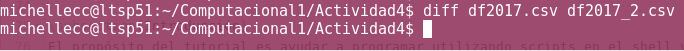
\includegraphics[height=6cm]{11.png}
\end{center}
\begin{center}
        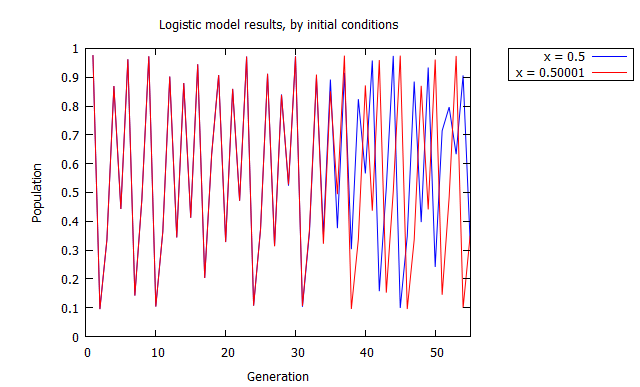
\includegraphics[height=3cm]{12.png}
\end{center}

Las gráficas realizadas son las mismas que se han estado trabajando.

\clearpage
Gráficas de fase, una para $x_1$ y otra para $x_2$.

\begin{figure}[h!]
\begin{subfigure}{.55\textwidth}
\centering
\includegraphics[width=1\linewidth]{ej4_1_1.png}
\end{subfigure}
\begin{subfigure}{.55\textwidth}
\centering
\includegraphics[width=1\linewidth]{ej4_1_2.png}
\end{subfigure}
\end{figure}

Plot de $x_1$ y $x_2$

\begin{figure}[h!]
\begin{subfigure}{.55\textwidth}
\centering
\includegraphics[width=1\linewidth]{ej4_1_3.png}
\end{subfigure}
\begin{subfigure}{.55\textwidth}
\centering
\includegraphics[width=1\linewidth]{ej4_1_4.png}
\end{subfigure}
\end{figure}

Como se mencionó, cuando se agrega fuerza, los primeros valores de t suelen mostrar alteraciones extrañas en el movimiento, mientras que para t más grande, se estabiliza. Para mostrar esto las siguientes gráficas utilizan t>110, mientras que las anteriores empiezan desde que t=0. \\

Para poder realizar esto, nos saltamos las primeras 550 líneas del archivo que creamos en un inicio:

\begin{center}
        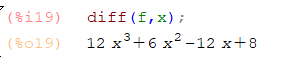
\includegraphics[height=7cm]{13.png}
\end{center}

Así pues creamos limit cycles (gráficas de fase):

\begin{figure}[h!]
\begin{subfigure}{.55\textwidth}
\centering
\includegraphics[width=1\linewidth]{ej4_1_5.png}
\end{subfigure}
\begin{subfigure}{.55\textwidth}
\centering
\includegraphics[width=1\linewidth]{ej4_1_6.png}
\end{subfigure}
\end{figure}

El movimiento de $x_1$ y $x_2$ con respecto al tiempo

\begin{center}
        \includegraphics[height=6cm]{ej4_1_7.png}
\end{center}

\cleardoublepage
Plot de $x_1$ vs $x_2$.

\begin{center}
        \includegraphics[height=6cm]{ej4_1_8.png}
\end{center}

\end{itemize}
\end{itemize}


\section{Conclusiones}

Agregando a las conclusiones de la semana pasada, reitero que me agradó mucho el ambiente de Jupyter Lab, bastante completo. \\ 

Por otro lado, al respecto del artículo, creo que esta semana se puso más interesante, se volvió un mayor reto, puesto que la semana pasada únicamente nos dedicamos a entender el código y modificar pequeñas partes, esta semana si cambiamos algo significativo y se creó un código que es flexible para cualquiera de los casos mencionados con anterioridad. \\

Me llamó mucho la atención que las gráficas resultantes fueran idénticas a los modelos analíticos, lo que nos dice que estos modelos nos dan una aproximación bastante buena.

\section{Bibliografía}

\begin{itemize}
\item Ley de elasticidad de Hooke (2018). Consultado: 25 de Marzo del 2018, de Wikipedia. Sitio web: https://es.wikipedia.org/wiki/Ley\_de\_elasticidad\_de\_Hooke
\item Couple spring equations (2003).Temple H. Fay, Sarah Duncan Graham. Consultado: 27 de Marzo del 2018, de Oregon State University. Sitio web:  http://math.oregonstate.edu/\\
\~gibsonn/Teaching/MTH323-010S15/Supplements/coupled\_spring.pdf
\end{itemize}

\section{Apéndice}

\begin{enumerate}
\item ¿Qué más te llama la atención de la actividad completa? ¿Que se te hizo menos interesante?

Me gustó mucho que nosotros pudieramos modificar y analizar el código para acomodarlo a nuestras necesidades.

\item ¿De un sistema de masas acopladas como se trabaja en esta actividad, hubieras pensado que abre toda una nueva área de fenómenos no lineales?

No, nunca me hubiera imaginado esto, puesto que en clase cuando analizamos este tipo de sistemas siempre nos vamos a lo más idealizado y no profundizamos al respecto.

\item ¿Qué propondrías para mejorar esta actividad? ¿Te ha parecido interesante este reto?

Me parece que ya tiene lo necesario, aunque siempre realizamos lo mismo, las pequeñas variaciones nos permiten dar el análisis físico.

\item ¿Quisieras estudiar mas este tipo de fenómenos no lineales?

Si me parece interesante, sin embargo, por el momento no me encuentro muy familiarizada al respecto.

\end{enumerate}
\end{document}